\chapter{Distributed Consensus}
\label{chpr:consensus}

\bigskip
\section{Distributed Systems}
With the persistent expansion of technology in the digital age we are going through, distributed systems are becoming more and more widespread.

\bigskip
\noindent
On one side big companies operate on a global scale with thousands of machines deployed all over the world, big data are stored in various data centers and computational power is shared on multi-core processors or computing clusters.

\bigskip
\noindent
On the other side, every day thousands of people withdraw money in a ATM point, a perfect example of distributed system. But simply, just think about a modern smartphone: it can share multiple data on the cloud and contain multiple co-working processing devices.

\bigskip
\noindent
However, there is no a unique formal definition of distributed system. The one that fits better our interest is:
\begin{mydef} {\bf (distributed system)\footnote{\url{https://en.wikipedia.org/wiki/Distributed_computing}}}.
    A distributed system is a system whose components are located on different networked computers, which communicate and coordinate their actions by passing messages to one another. The components interact with one another in order to achieve a common goal. Three significant characteristics of distributed systems are: concurrency of components, lack of a global clock, and independent failure of components.
\end{mydef}

\bigskip
\noindent
Therefore, the main reasons for using distributed systems are:
\begin{itemize}
    \item Scalability: Distributed systems should be scalable with respect to geography, administration or size.
    \item Performance: Compared to other models, distributed models are expected to give a higher boost to performance.
    \item Fault Tolerance: A cluster of multiple machines is inherently more fault-tolerant than a single source of failure.
    \item Reliability: Data is replicated on different machines in order to prevent loss.
    \item Availability: Data is replicated on different machines to minimize latency and provide faster access.
\end{itemize}

\bigskip
\noindent
However, beautiful features like these often have a downside, bringing to light some challenging problems:
\begin{itemize}
    \item Security: Especially when networks are public.
    \item Coordination\footnote{In the fin-tech industry, coordination problems come with various names: consistency, agreement, consensus or Blockchain.}: In public distributed systems coordination problems are prevalent if proper protocols or policies are not in place; agents could be malevolent or malicious.
\end{itemize}
Thus, it can be easily inferred that one of the main challenges of distributed systems is to achieve overall system reliability in the presence of a number of faulty processes. Examples of applications of consensus include whether to commit a transaction to a database, agreeing on the identity of a leader, state machine replication, clock synchronization, PageRank, load balancing and many others. Let us get in a detailed study of what consensus is and how consensus can be achieved in a distributed system.

\bigskip
\section[The Consensus Problem]{The Consensus Problem\footnote{Definitions and Algorithms presented in this section are taken from \cite{Wattenhofer:2016:SB:3002702}, a book in which the author deeply delves into the problem of achieving consensus in distributed systems.}} 
Networks are composed by many agents, called \textit{nodes}. Think of a computer network, nodes are either \textit{honest}, executing programs faithfully, or \textit{byzantine} \cite{Lamport:1982:BGP:357172.357176}, exhibiting arbitrary behavior. We will also define them \textit{correct} and \textit{faulty}, but not as alternatives to honest and byzantine. A correct node is an honest node that always eventually makes progress. A faulty node is a Byzantine node or an honest node that has crashed or will eventually crash. Note that honest and Byzantine
are mutually exclusive, as are correct and faulty. However, a node can be both honest and faulty.
\begin{mydef} {\bf (node)}.
    We call a single actor in the system node. In a computer network the computers are the nodes, in the classical client-server model both the server and the client are nodes, and so on.
\end{mydef}
\begin{mydef} {\bf (byzantine node)\footnote{Before the term \textit{byzantine} was coined, the terms Albanian Generals or Chinese Generals were used in order to describe malicious behavior. When the involved researchers met people from these countries they moved, for obvious reasons, to the historic term byzantine.}}.
    \label{def:byzantine-node}
    A node which can have arbitrary behaviour is called byzantine. This includes \enquote{anything imaginable}, e.g., not sending any massage at all, or sending different and wrong messages to different neighbors, or lying about the input value.
\end{mydef}

\bigskip
\noindent
We assume that each pair of nodes is connected by a link, which is a bi-directional reliable virtual circuit
and therefore messages sent on this link are delivered, eventually, and in the order in which they were sent
(i.e., an honest sender keeps retransmitting a message until it receives an acknowledgment or crashes). A
receiver can tell who sent a message (e.g., using MACs), so a Byzantine node cannot forge a message so it
is indistinguishable from a message sent by an honest node.

\bigskip
\noindent
In the consensus problem nodes run \textit{actors}, that are either \textit{proposers}, each of which proposes a \textit{proposal}, or \textit{deciders}, each of which \textit{decides} one of the proposals. Assuming there exists at least one correct proposer
(i.e., a proposer on a correct node), the goal of a consensus protocol is to ensure each correct decider decides
the same proposal, even in the face of faulty proposers. A node may run both a proposer and a decider, in
practice a proposer often would like to learn the outcome of the agreement.
\begin{mydef} {\bf (consensus)}.\label{def:consensus}
    There are $n$ nodes, of which at most $f$ might crash, i.e., at least $n-f$ nodes are correct. Node $i$ starts with a proposed value $v_{i}$. The nodes must decide for one of those values, satisfying the following properties:
    \begin{itemize}
        \item Agreement: All correct nodes decide for the same proposal.
        \item Termination: All correct nodes terminate in finite time.
        \item Validity: The decision value must be the proposal of some proposer.
    \end{itemize}
\end{mydef}

\bigskip
\noindent
What is really interesting is to learn how to achieve distributed consensus in an asynchronous network in presence of byzantine nodes. Starting with the historical formulation of the problem and a first example of solved consensus in a model that is synchronous, we will finally face a famous impossibility result in the asynchronous case.

\bigskip
\subsection{The Byzantine Generals' Problem}
Distributed computer systems that want to be reliable must handle faulty components that give conflicting information to different parts of the system.

\bigskip
\begin{figure}[h]
    \centering
	
\includegraphics[width=0.9\linewidth]{Images/byzantine.jpeg}
	\caption{Conquest of Constantinople}
	\label{fig:figure4}
	\source{\url{https://medium.com/all-things-ledger/the-byzantine-generals-problem-168553f31480}}
\end{figure}

\bigskip
\noindent
The \enquote{Byzantine Generals' Problem} is the abstraction of the aforementioned situation.
We imagine that several divisions of the Byzantine army are camped outside an enemy city, each division commanded by its own general. The generals communicate with one another as well as with all lieutenants only by messenger. After observing the enemy, they must decide upon a common plan of action: the exact time to attack all at once or, if faced by fierce resistance, the time to retreat all at once. The army cannot hold on forever, if the attack or retreat is without full strength then brutal defeat is the only possible outcome. However, some of the generals may be traitors, trying to prevent loyal generals from reaching agreement. 

\bigskip
\noindent
For simplicity, we can restrict ourselves to the case of a commanding general sending an order to his lieutenants, obtaining the following problem.
\begin{mydef}{\bf (byzantine generals' problem)}.
\label{def:bgp}
    A commanding general must send an order to his $n-1$ lieutenant generals such that the following conditions\footnote{Conditions \ref{cond:1} and \ref{cond:2} are called the \textit{interactive consistency} conditions} are satisfied:
    \begin{enumerate}
        \item \label{cond:1} All loyal lieutenants obey the same order.
        \item \label{cond:2} If the commanding general is loyal, then every loyal lieutenant obeys the order he sends.
    \end{enumerate}
\end{mydef}

\bigskip
\subsection{Byzantine Agreement}
Achieving consensus (as in Definition \ref{def:consensus}) in a system with byzantine nodes is hard stuff. A careful reader immediately realizes that fulfilling agreement and termination is straight-forward, but what about validity? Reminding that a byzantine node can be malevolent lying about its input value, we must specify different types of validity:
\begin{mydef}{\bf (any-input validity)\footnote{This is the validity definition we implicitly used for consensus, in Definition \ref{def:consensus}}}.
    The decision value must be the proposed value of any node.
\end{mydef}
\noindent
As we can see, this definition does not still make sense in presence of byzantine nodes; we would wish for a differentiation between byzantine and correct inputs.
\begin{mydef}{\bf (correct-input validity)}.
    The decision value must be the proposed value of a correct node.
\end{mydef}
\noindent
Fulfilling this particular validity definition is not so simple, as byzantine nodes following correctly a specified protocol but lying about theirs input values are indistinguishable from correct nodes. An alternative could be:
\begin{mydef}{\bf (all-same validity)}.
    If all correct nodes start with the same proposed value $v$, the decision value must be $v$.
\end{mydef}
\noindent
Here, if the decision values are binary, then correct-input validity is induced by all-same validity. Else, if the input values are not binary, all-same validity is not useful anymore.

\bigskip
\noindent
Now that we have clear in mind what are the ingredients for the consensus recipe, a question bales to us: which are the algorithms that solve byzantine agreement? What type of validity they fulfill? The King algorithm is one of the best examples, but we have to restrict ourselves to the so-called synchronous model.
\begin{mydef}{\bf (synchronous model)}.
    In the synchronous model, nodes operate in synchronous rounds. In each round, each node may send a message to the other nodes, receive the message sent by the other nodes, and do some local computation.
\end{mydef}

\begin{algorithm}
	\caption{King Algorithm (for $f<n/3$)}
	\label{alg:king}
	\begin{algorithmic}[1]
		\State $x =$ my input value
		\For {phase $= 1$ to $f+1$}
		\Statex \ \ \ \ \textit{Round 1}
		\State Broadcast $value(x)$
		\Statex \ \ \ \ \textit{Round 2}
		\If {some $value(y)$ at least $n-f$ times}
		\State Broadcast $propose(y)$
		\EndIf 
		\If {some $propose(z)$ received more than $f$ times}
		\State $x=z$
		\EndIf
		\Statex \ \ \ \ \textit{Round 3}
		\State Let node $v_{i}$ be the predefined king of this phase $i$
		\State The king $v_{i}$ broadcasts its current value $w$
		\If {received strictly less than $n-f$ $propose(x)$}
		\State $x=w$
		\EndIf
		\EndFor
	\end{algorithmic}
\end{algorithm}

\newpage

\bigskip
\noindent
To be rigorous, we must state some useful lemmas in order to prove that Algorithm \ref{alg:king} solves byzantine agreement.
\begin{mylemma}
    \label{lemma:1}
    Algorithm \ref{alg:king} fulfills the all-same validity.
\end{mylemma}
\begin{mylemma}
    \label{lemma:2}
    There is at least one phase with a correct king.
\end{mylemma}
\begin{mylemma}
    \label{lemma:3}
    After a round with a correct king, the correct nodes will not change their values $v$ anymore, if $n > 3f$.
\end{mylemma}

\begin{thm}
    Algorithm \ref{alg:king} solves byzantine agreement.
\end{thm}
\begin{proof}
    The king algorithm reaches agreement as either all correct nodes start with the same value, or they agree on the same value latest after the phase where a correct node was king according to Lemmas \ref{lemma:2} and \ref{lemma:3}. Because of Lemma \ref{lemma:1} we know that they will stick with this value. Termination is guaranteed after $3(f+1)$ rounds, and all-same validity is proved in Lemma \ref{lemma:1}.
\end{proof}

\bigskip
\noindent
However, this is not the end of the story about distributed consensus. In order to dig into the hearth of this work we must introduce consensus results in the asynchronous model.
\begin{mydef}{\bf (asynchronous model)}.
    In the asynchronous model, algorithms are event based (\enquote{upon receiving message ..., do ...}). Nodes do not have access to a synchronized wall-clock. A message sent from one node to another will arrive in a finite but unbounded time.
\end{mydef}
\begin{mydef}{\bf (asynchronous runtime)}.
    For algorithms in the asynchronous model, the runtime is the number of time units from the start of the execution to its completion in the worst case (every legal input, every execution scenario), assuming that each message has a delay of at most one time unit.    
\end{mydef}

\bigskip
\noindent
We will now present a famous algorithm (Algorithm \ref{alg:ben-or}) by Ben-Or \cite{Ben-Or:1983:AFC:800221.806707}, which tries to solve asynchronous byzantine agreement.

\bigskip
\begin{algorithm}
	\caption{Asynchronous Byzantine Agreement (Ben-Or, for $f < n/9$)}
	\label{alg:ben-or}
	\begin{algorithmic}[1]
		\State $x_{i} \in \{0,1\}$ \Comment{input bit}
		\State $r=1$ \Comment{round}
		\State decided = false
		\State Broadcast $propose(x_{i},r)$
		\Repeat
		\State Wait until $n-f$ $propose$ messages of current round $r$ arrived
		\If{at least $n-2f$ $propose$ messages contain the same value $x$}
		\State $x_{i}=x$, decided = true
		\ElsIf{at least $n-4f$ $propose$ messages contain the same value $x$}
		\State $x_{i}=x$
		\Else
		\State choose $x_{i}$ randomly, with $Pr[x_{i}=0] = Pr[x_{i}=1] = 1/2$
		\EndIf
		\State $r=r+1$
		\State Broadcast $propose(x_{i},r)$
		\Until{decided (see Line 8)}
		\State decision = $x_{i}$
	\end{algorithmic}
\end{algorithm}

\bigskip
\noindent
Unfortunately, Algorithm \ref{alg:ben-or} is just a proof of concept that asynchronous byzantine agreement can be achieved, but practically it is unfeasible due to its exponential runtime.

\bigskip
\subsection{Impossibility Result}
A solution to the Byzantine Generals' Problem \ref{def:bgp} may seem a piece of cake. That's not true at all. Its difficulty arises from the fact that if the generals can send only oral messages, then no solution will work unless more than two-thirds of the generals are loyal. An oral message is one whose contents are completely under the control of the sender, so a traitorous sender can transmit any possible message.
Such a message corresponds to the type of message that computers normally send to one another.

\bigskip
\noindent
Let us now show that, if only oral messages are allowed, there is no solution for three generals with a single traitor. For simplicity, the only possible messages that generals can send are \enquote{attack} or \enquote{retreat}. This restriction opens two possible scenarios. In the first scenario, shown in Figure \ref{fig:scenario1}, a loyal commander sends an \enquote{attack} order to his lieutenants, but lieutenant 2 is malevolent and report \enquote{retreat} to lieutenant 1. In this situation, in order to satisfy Condition \ref{cond:2} of problem \ref{def:bgp}, lieutenant 1 must obey the order to attack. In the second scenario, shown in Figure \ref{fig:scenario2}, the commander is a traitor and sends an \enquote{attack} command to lieutenant 1, and a \enquote{retreat} order to lieutenant 2. But, lieutenant 1 does not know who is the traitor and cannot tell the order the commander sent to lieutenant 2. Thus, lieutenant 1 cannot distinguish in which scenario he belongs, so he always obey to the \enquote{attack} order. With a similar argument, if lieutenant 2 receive a \enquote{retreat} order from the commander, he must follow him even if lieutenant 1 reports him to attack. This violates Condition \ref{cond:1} of problem \ref{def:bgp}.

\begin{figure}
\centering
\begin{minipage}{.5\textwidth}
  \centering
  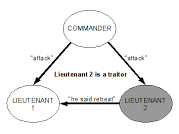
\includegraphics[width=.8\linewidth]{Images/scenario1.png}
  \captionof{figure}{Lieutenant 2 is a traitor}
  \label{fig:scenario1}
\end{minipage}%
\begin{minipage}{.5\textwidth}
  \centering
  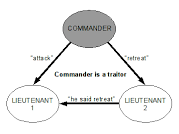
\includegraphics[width=.8\linewidth]{Images/scenario2.png}
  \captionof{figure}{Commander is a traitor}
  \label{fig:scenario2}
\end{minipage}
\source{\url{https://www.researchgate.net/figure/Byzantine-Generals-Problem-Lamport82_fig4_263046309}}
\end{figure}

\bigskip
\noindent
A demanding reader could comply about this nonrigorous result. A famous result\footnote{This result was awarded the 2001 PODC Influential Paper Award (now called Dijkstra Prize).} of Fisher, Lynch and Paterson \cite{Fischer:1985:IDC:3149.214121} formally proves impossibility of distributed consensus with one faulty process.

\bigskip
\noindent
Due to this proven impossibility result, how Satoshi Nakamoto reaches consensus in Bitcoin, a decentralized, distributed, peer-to-peer network? In the next chapter we will delve into this argument.